\documentclass[a4paper,12pt]{scrartcl}
\usepackage{hyperref}
\usepackage{url}            % simple URL typesetting
\usepackage{booktabs}       % professional-quality tables
\usepackage{amsfonts}       % blackboard math symbols
\usepackage{amsmath}
\usepackage{nicefrac}       % compact symbols for 1/2, etc.
\usepackage{microtype}      % microtypography
\usepackage{tabto}
\usepackage{tikz}
\usepackage{graphicx}
\usepackage{longtable}
\usepackage{lmodern}
\usepackage{listings}
\usepackage[T1]{fontenc}
\usepackage[utf8]{inputenc}
\usepackage{forest}
\definecolor{folderbg}{RGB}{124,166,198}
\definecolor{folderborder}{RGB}{110,144,169}

\def\Size{4pt}
\tikzset{
  folder/.pic={
    \filldraw[draw=folderborder,top color=folderbg!50,bottom color=folderbg]
      (-1.05*\Size,0.2\Size+5pt) rectangle ++(.75*\Size,-0.2\Size-5pt);  
    \filldraw[draw=folderborder,top color=folderbg!50,bottom color=folderbg]
      (-1.15*\Size,-\Size) rectangle (1.15*\Size,\Size);
  }
}




\title{,,ROZPOZNAWANIE KOTKÓW OD PIESKÓW''}
\author{Michał Skibiński (260352)}
\date{30.05.2022}

\begin{document}

\maketitle

\renewcommand*\contentsname{spis treści}
\tableofcontents
\newpage{}

\section{Wstęp}
\subsection{cel projektu}
Przedmiotem projektu jest zadanie klasyfikacji binarnej (klasyfikacji kotów oraz psów).
\subsection{narzędzia}
\begin{itemize}
\item problem rozwiązany został za pomocą  \textbf{konwolucyjnej sieci neuronowej (CNN)}.
Ponieważ sieci neuronowe operują na macierzach, są one szczególnie wydajne przy pracy z obrazami, 
które tak naprawde są macierzami pikseli. \\
\item Rozwiązanie zaprojektowane zostało w języku \textbf{python}, ze względu na jego prostotę, 
niezawodność oraz wielorakość bibliotek ogólno-dostępnych. \\
\item biblioteka użyta do rozwiązania problemu to \textbf{tensorflow}. Została ona użyta ze względu na możliwość 
wykonywania złożonych operacji na sieciach neuronowych, przy użyciu stosunkowo
niewielkiej ilości kodu. Oprócz tego biblioteka ta działa bardzo efektywnie,
 oraz została do niej napisana bogata dokumentacja.\\
\end{itemize}
\newpage{}
\section{Model}


\subsection{przygotowanie danych}
aby przygotować dane kolejno:
\begin{enumerate}

    \item zaprojektowany został algorytm do odczytywania zdjęć z zadanego folderu i tworzeniu folderu plików z podziałem na \textbf{dane testowe i treningowe} oraz klasy, tak by strukrura wyglądała następująco: \\
    \begin{forest}
        for tree={
          font=\ttfamily,
          grow'=0,
          child anchor=west,
          parent anchor=south,
          anchor=west,
          calign=first,
          inner xsep=7pt,
          edge path={
            \noexpand\path [draw, \forestoption{edge}]
            (!u.south west) +(7.5pt,0) |- (.child anchor) pic {folder} \forestoption{edge label};
          },
          before typesetting nodes={
            if n=1
              {insert before={[,phantom]}}
              {}
          },
          fit=band,
          before computing xy={l=15pt},
        }  
      [input for model
        [train
          [cats (3830 zdjęć)
          ]
          [dogs (1915 zdjęć)
          ]
        ]
        [test
            [cats (958 zdjęć)
            ]
            [dogs (479 zdjęć)
            ]
        ]
      ]
      \end{forest}\\
      ilość danych testowych zdefiniowana została na 20 procent wszystkich danych.
    \item usunięta została różnica w ilości fotografii kotów i psów (ważne aby sieć neuronowa miała tyle samo danych z każdej z klas) 
    \item dokonana została \textbf{normalizacji danych} -  wartości pikseli zostały przeskalowane, tak by pochodziły z zakresu [0,1)
    \item dokonana została standaryzacja danych - wszystkie zdjęcia przeskalowane zostały do rozmiarów [224 x 224] px.
    \item redukcja wymiarów danych przy użyciu \textbf{PCA} nie została zastosowana, ponieważ wiązała się ze zbyt dużą utratą danych. 
      
  \end{enumerate}
\subsection{budowa modelu}
model inspirowany jest dotychczasowymi modelami do rozwiązania tego typu problemów.
Zanim pojawił się finałowy model stworzone zostało ok 10 innych modeli, każdy był usprawnieniem poprzedniego.
przy udoskonalaniu modelu, nacisk kładziony był na zamianie \textbf{funkcji aktywujących} dla poszczególnych warstw oraz liczbie ich liczbie.\\\\

włsności modelu:
\begin{itemize}
  \item wejście dla modelu: macierz o rozmiarach (224 x 224 x 3) - gdzie 3 wynika z reprezentacji pikseli poprzez RGB 
  \item liczba warstw ukrytych: 20 
  \item wyjście: wartość 0 lub 1 (0 - dla psa, 1 - dla kota) 
  \item metoda optymalizacji:  \textbf{stochastyczny spadek gradientu(SGD)} z prędkością nauki = 0.0001
  \item funkcja strat:  binarna entropia krzyżowa
  \item ilość generacji(epok):  20
  \item populacja w każdej generacji: 60
  \item \textbf{funkcja regularyzacji}: l2 (bez regularyzacji występowało \textbf{przetrenowanie modelu})
\end{itemize}  

\subsection{przebieg treningu}

\begin{figure}[h]
  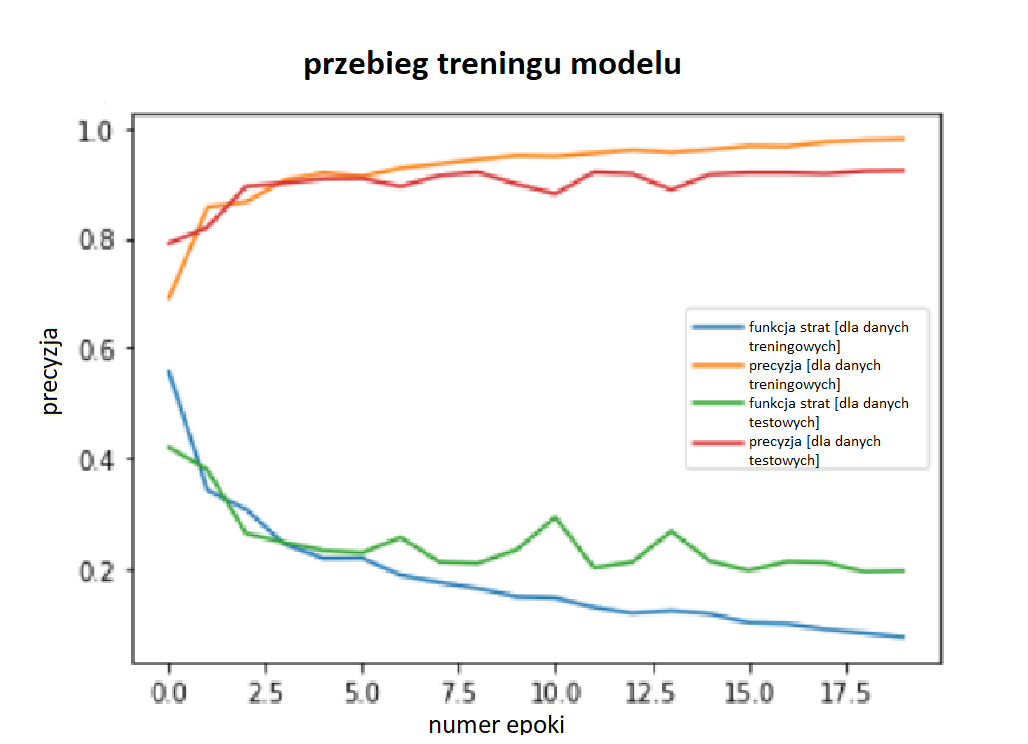
\includegraphics[width=\linewidth]{TRENINNG.png}
\end{figure}
\newpage{}
\section{Wyniki}
\subsection{kryterium jakości modelu}
jakość modelu mierzona została ze względu na \textbf{precyzję}.
kryterium to zostało wybrane, ze względu na jego prostotę,
precyzja jest dobrą metryką do 
oceny wydajności modelu w prostych modelach, takich jak ten.\\\\
$precyzja = \frac{ilość\ poprawnie\ sklasyfikowanych\ zdjęć}{ilość\ wszystkich\ zdjęć} * 100 \% $\\\\
$przecyzja \in [0 \ \% \ , 100 \ \% \ ] \ $ - im wyższa tym lepsza

\subsection{jakość modelu}

po skończonym treningu precyzja:
\begin{itemize}
  \item dla danych treningowych wynosiosła: \textbf{98 procent}
  \item dla danych testowych: \textbf{93 procent}
\end{itemize}

Do przedstawienia graficznie precyzji dla danych testowych
modelu  użyta zotsała macierz pomyłek (confusion matrix).\\
gdzie:
\begin{itemize}
  \item 0 - etykieta dla \textit{psa}
  \item 1 - etykieta dla \textit{kota}
\end{itemize}
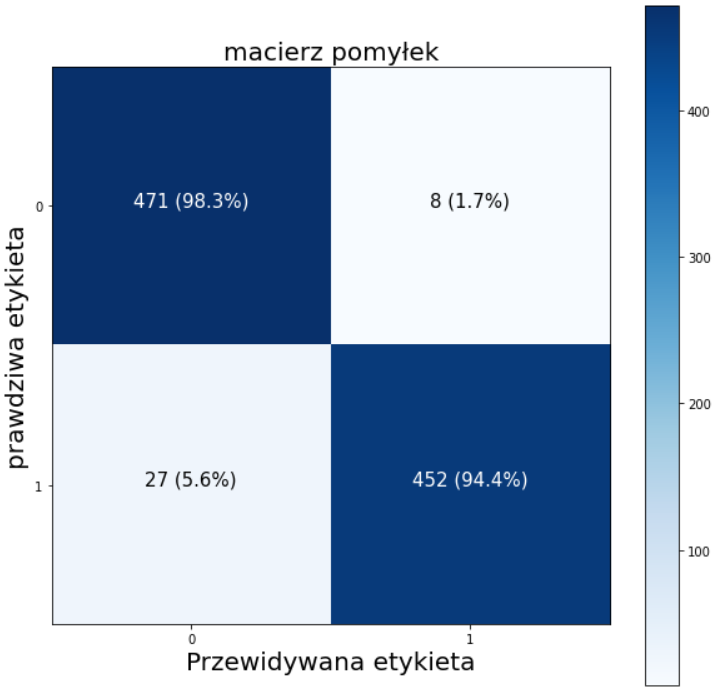
\includegraphics[scale=0.5]{conf.png}\\
Jak widać model ma większe trudności z poprawnym zaklasyfikowaniem kotów niż psów.
Prawie 6 \%  kotów zostało sklasyfikowanych jako psy - a tylko niecałe 2 \% psów zostało błędnie sklasyfikowanych jako koty  

Aby zweryfikować poprawność modelu uruchominy on został dla zdjęć zrobionych przeze mnie oraz moich znajomych,
tak aby mieć pewność że zdjęcia są różnych formatów, rozmiarów, różnej jakości i nie 
były wcześniej w żaden sposób przerobione
\begin{figure}[h]
  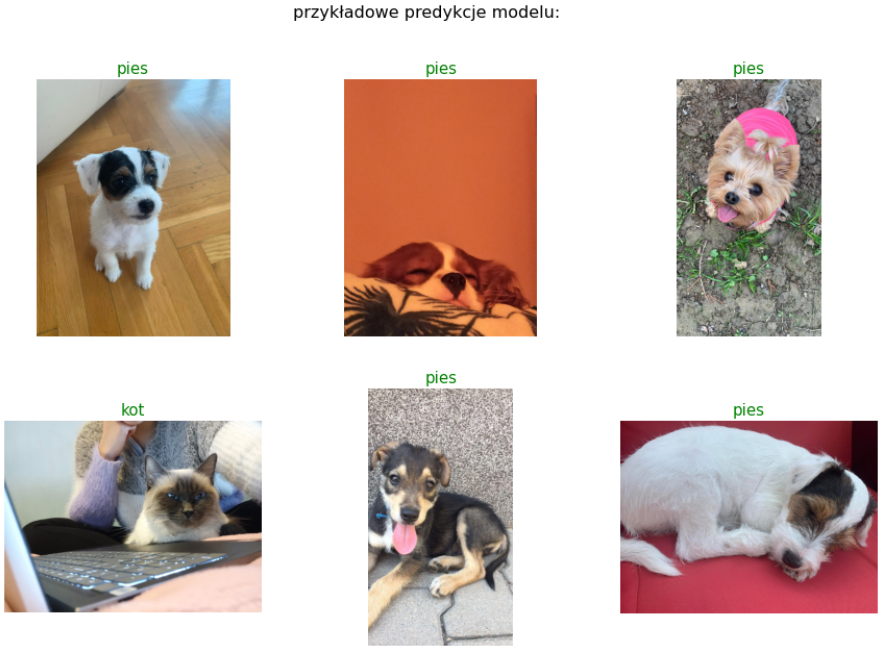
\includegraphics[width=\linewidth]{preedictions.png}
\end{figure}
\newpage{}
\subsection{przyczyny takiej a nie innej jakość modelu}
model okazał się stosunkowo skuteczny, przy klasyfikacji 
zdjęć nie spreparowanych skuteczność na poziomie 93 
procent, możemy uznać za zadowalającą.\\\\
\textbf{dlaczego model nie ma skuteczności na poziomie 100 procent?}\\
\begin{enumerate}
  \item ponieważ urządzenie na którym prowadzone było trenowanie modelu dysponowało niewielkią mocą obliczeniową,
   a operacje na zdjęciach, są skomplikowane - trenowanie sieci zakończone zostało gdy jej dokładość miała dalej tendencje 
   rosnące.
  \item niektóre ze zdjęć mogły być nieostre, lub przedstawiać zwierzę które jest mieszanką genetyczną psa i kota.
  przykład takich zdjęć: 
  \begin{figure}[h]
    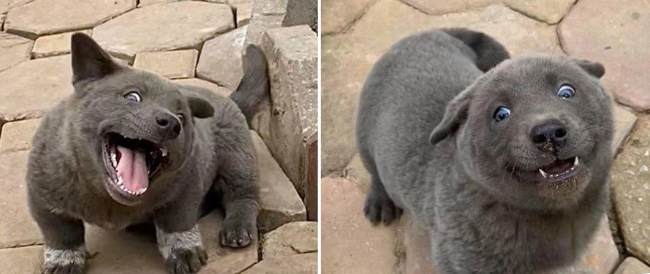
\includegraphics[width=\linewidth]{example.png}
  \end{figure}
\end{enumerate} 


\section{przypisy}
zdjęcia użyte do budowy dla modelu:\\ 
\href{https://www.kaggle.com/datasets/zippyz/cats-and-dogs-breeds-classification-oxford-dataset}
{https://www.kaggle.com/datasets/zippyz/cats-and-dogs-breeds-classification-oxford-dataset}
kod rozwiązania:\\
\href{https://github.com/michalskibinski109/projekt/blob/main/PROJEKT.ipynb}
{https://github.com/michalskibinski109/projekt/blob/main/PROJEKT.ipynb}

\end{document}

